\documentclass[a4paper, 12pt]{article}
\usepackage[utf8x]{inputenc}
\usepackage{cmap}
\usepackage[english, russian]{babel}
\usepackage{indentfirst}
\usepackage[left=20mm, top=20mm, right=20mm, bottom=20mm]{geometry}
\usepackage{tikz}
\usepackage{float}
\usepackage{amsmath, amsfonts, amssymb}
\usepackage{graphicx}
\usepackage{fancybox, fancyhdr}
\usepackage{hyperref}
\usepackage{listings}
\usepackage{caption}
\usepackage{subcaption}
\usepackage{xcolor}
\pagestyle{fancy}
\fancyhf{}
\fancyhead[L]{Лабораторная работа №5}
\fancyhead[R]{Частотные методы}
\fancyfoot[C]{\thepage}
\graphicspath{{images/}}
\usetikzlibrary{patterns}
\definecolor{LightGray}{gray}{0.95}
\definecolor{LightGray2}{gray}{0.7}
\lstdefinestyle{code}{
    language=Python,
    basicstyle=\footnotesize\ttfamily,
    numbers=left,
    numberstyle=\scriptsize\color{gray},
    stepnumber=1,
    numbersep=5pt,
    backgroundcolor=\color{LightGray},
    showspaces=false,
    showstringspaces=false,
    showtabs=false,
    tabsize=4,
    captionpos=b,
    breaklines=true,
    breakatwhitespace=false,
    frame=single,
    rulecolor=\color{LightGray2},
    linewidth=\linewidth,
    keywordstyle=\color{blue}\bfseries,
    commentstyle=\color{green!40!black},
    stringstyle=\color{purple},
    escapeinside={\%*}{*)},
    inputencoding=utf8x,
    xleftmargin=0pt,
    framexleftmargin=0pt,
    framexrightmargin=0pt
}
\lstset{style=code}
\hypersetup{
    colorlinks=true,
    linkcolor=blue,
    filecolor=magenta,
    urlcolor=cyan,
    pdftitle={contents setup},
    pdfpagemode=FullScreen,
}
\setlength{\parskip}{1.5mm}
\setlength{\headheight}{15pt}
\setlength{\footskip}{15pt}
\allowdisplaybreaks
\DeclareMathOperator{\sinc}{sinc}
\newcommand{\frc}[2]{\raisebox{2pt}{$#1$}\big/\raisebox{-3pt}{$#2$}}

\begin{document}
    \begin{titlepage}

        \begin{center}
        
\includegraphics[width=0.3\textwidth]{itmo.png} % requires itmo.png in /images folder
        \vfill

        Федеральное государственное автономное образовательное учреждение высшего образования
        «Национальный Исследовательский Университет ИТМО»\\

        \vfill
        {\large\bf ЛАБОРАТОРНАЯ РАБОТА №5}\\
        {\large\bf ПРЕДМЕТ «ЧАСТОТНЫЕ МЕТОДЫ»}\\
        {\large\bf ТЕМА «СВЯЗЬ НЕПРЕРЫВНОГО И ДИСКРЕТНОГО»}
        \vfill

        \begin{flushright}
            \begin{minipage}{.45\textwidth}
            {
                \hbox{Лектор: Перегудин А. А.}
                \hbox{Практик: Пашенко А. В.}
                \hbox{Студент: Румянцев А. А.}
                \hbox{Поток: ЧАСТ.МЕТ. 1.3}
                \hbox{}
                \hbox{Факультет: СУиР}
                \hbox{Группа: R3241}
            }
            \end{minipage}
        \end{flushright}

        \vfill

        Санкт-Петербург\\
        2024
        \end{center}
    \end{titlepage}

    \tableofcontents

    \newpage
    \section{Задание 1. Непрерывное и дискретное преобразование Фурье}
    Рассмотрим прямоугольную функцию $\Pi:\mathbb{R}\rightarrow\mathbb{R}$:
    $$\Pi(t)=
    \begin{cases}
        1, & |t| \leq \frc{1}{2},\\
        0, & |t| > \frc{1}{2}.
    \end{cases}$$


    \subsection{Истинный Фурье-образ}
    Найдем аналитическое выражение для Фурье-образа прямоугольной функции
    $$\hat{\Pi}(\nu)=\int\limits_{-\infty}^{+\infty}\Pi(t)e^{-2\pi i \nu t}\,dt=\int\limits_{-\frac{1}{2}}^{\frac{1}{2}}e^{-2\pi i \nu t}\,dt
    =-\dfrac{e^{-\pi i \nu}-e^{\pi i \nu}}{2\pi i\nu}=\dfrac{\sin{\left(\pi\nu\right)}}{\pi\nu}=\sinc{\left(\nu\right)}$$
    Построим графики $\Pi(t)$ и $\hat{\Pi}(\nu)$
    \begin{figure}[H]
        \centering
        \begin{subfigure}{0.45\textwidth}
            \centering
            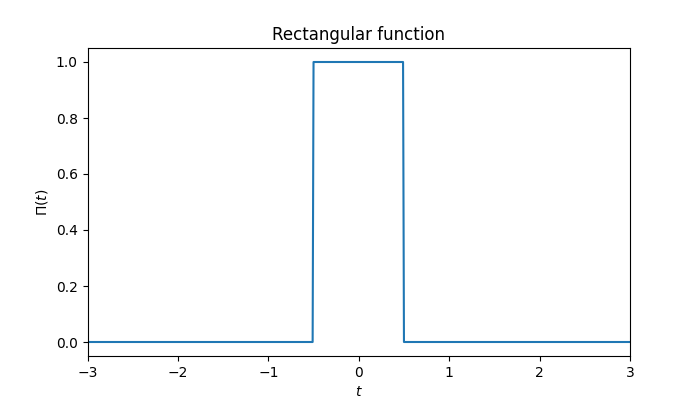
\includegraphics[width=\linewidth]{rectf.png}
            \caption{Прямоугольная функция}
            \label{fig:rectf}
        \end{subfigure}
        \hspace{5mm}
        \begin{subfigure}{0.45\textwidth}
            \centering
            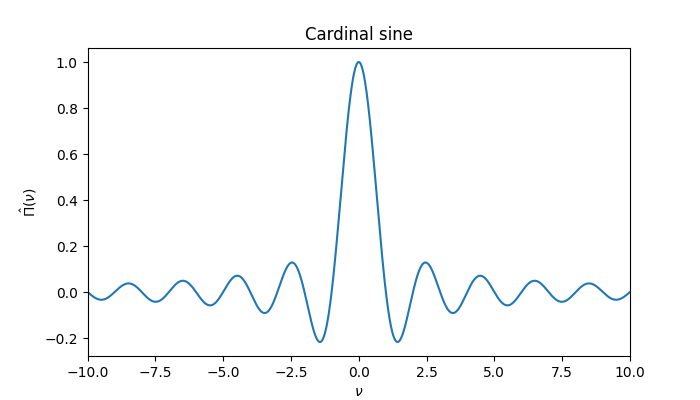
\includegraphics[width=\linewidth]{sinc.png}
            \caption{Кардинальный синус}
            \label{fig:sinc}
        \end{subfigure}
        \caption{Исходный сигнал и его Фурье-образ}
        \label{fig:rectfsinc}
    \end{figure}


    \subsection{Численное интегрирование}
    Зададим функцию $\Pi(t)$ в \texttt{Python}. Найдем ее Фурье-образ с помощью численного интегрирования (функция \texttt{trapz}).
    Вновь используя численное интегрирование, выполним обратное преобразование Фурье от найденного Фурье-образа с целью восстановить исходную функцию.
    Схематично наши действия будут выглядеть так:
    \begin{center}
        $\Pi(t)$
        \begin{tikzpicture}
            \draw[->] (0,0) -- (1,0) node[midway, above] {\tiny{\texttt{trapz}}};
        \end{tikzpicture}
        $\hat{\Pi}(\nu)$
        \begin{tikzpicture}
            \draw[->] (0,0) -- (1,0) node[midway, above] {\tiny{\texttt{trapz}}};
        \end{tikzpicture}
        $\Pi(t)$
    \end{center}
    Построим график найденной функции $\hat{\Pi}(\nu)$ и восстановленной функции $\Pi(t)$.
    Сравним результат с истинной функцией и Фурье-образом. Исследуем влияние
    величины шага интегрирования и размера промежутка, по которому вычисляется
    интеграл, на результат. Сделаем выводы о точности и быстродействии метода.


    Далее приведены соответствующие графики. Оранжевым цветом выделены оригинальные функции, синим --
    найденные через преобразования. Каждый график подписан сверху. Под временной шкалой также указаны
    рассматриваемый промежуток времени или частот и шаг дискретизации во временной или частотной областях.
    \begin{figure}[H]
        \centering
        \begin{subfigure}{0.45\textwidth}
            \centering
            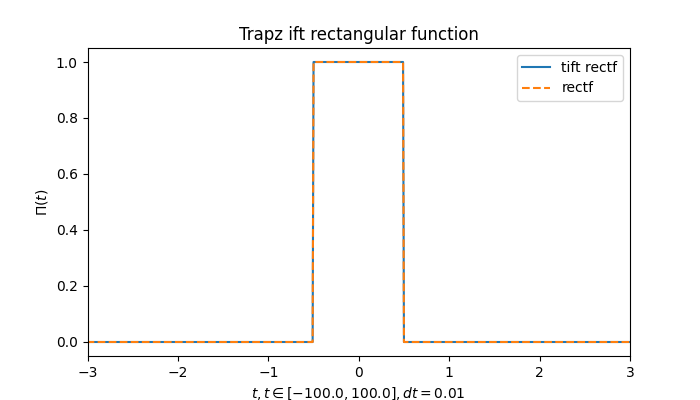
\includegraphics[width=\linewidth]{1_tiftr.png}
            \caption{$\Pi(t)$, восстановленная \texttt{trapz}}
            \label{fig:trectf1}
        \end{subfigure}
        \hspace{5mm}
        \begin{subfigure}{0.45\textwidth}
            \centering
            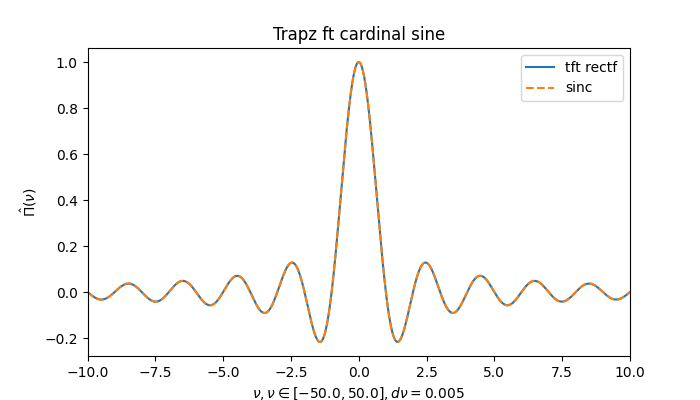
\includegraphics[width=\linewidth]{1_tftr.png}
            \caption{$\hat{\Pi}(t)$ восстановленной \texttt{trapz} $\Pi(t)$}
            \label{fig:tsinc1}
        \end{subfigure}
        \caption{Интеграл по всей области определения функции от $-100$ до $100$}
        \label{fig:trapzs1}
    \end{figure}
    \vspace{-5mm}
    \begin{figure}[H]
        \centering
        \begin{subfigure}{0.45\textwidth}
            \centering
            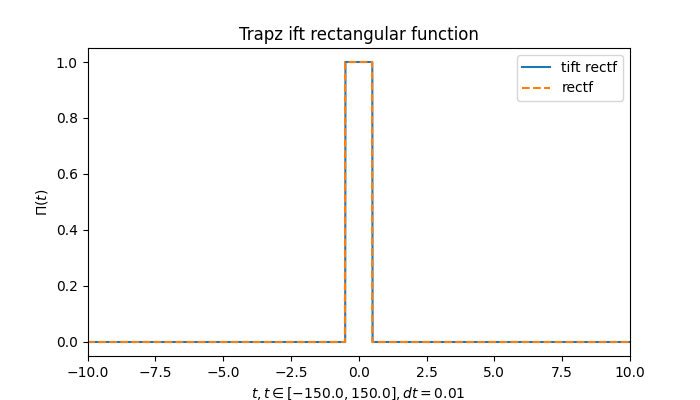
\includegraphics[width=\linewidth]{4_tiftr.png}
            \caption{$\Pi(t)$, восстановленная \texttt{trapz}}
            \label{fig:trectf4}
        \end{subfigure}
        \hspace{5mm}
        \begin{subfigure}{0.45\textwidth}
            \centering
            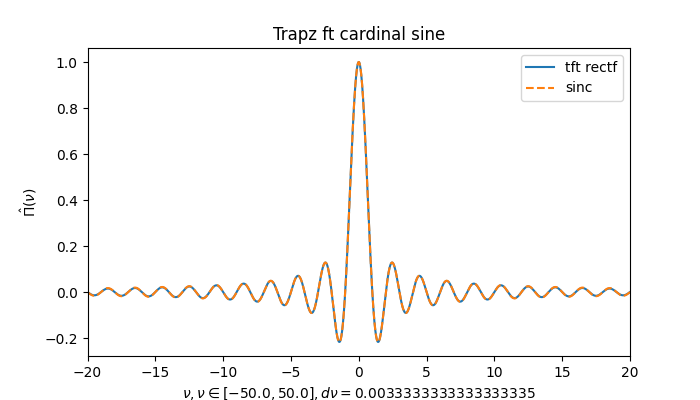
\includegraphics[width=\linewidth]{4_tftr.png}
            \caption{$\hat{\Pi}(t)$ восстановленной \texttt{trapz} $\Pi(t)$}
            \label{fig:tsinc4}
        \end{subfigure}
        \caption{Интеграл на увеличенном промежутке от $-150$ до $150$}
        \label{fig:trapzs4}
    \end{figure}
    \vspace{-5mm}
    \begin{figure}[H]
        \centering
        \begin{subfigure}{0.45\textwidth}
            \centering
            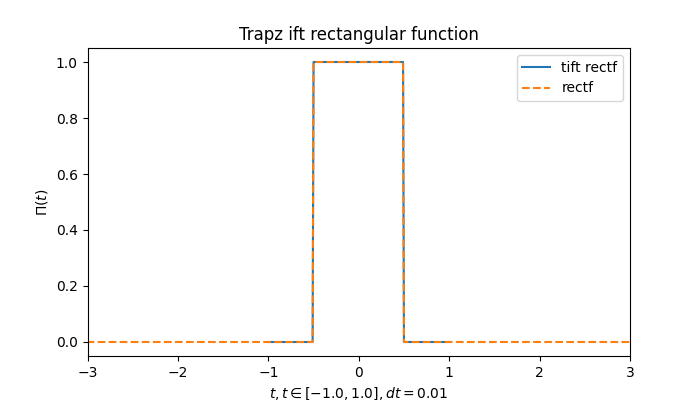
\includegraphics[width=\linewidth]{2_tiftr.png}
            \caption{$\Pi(t)$, восстановленная \texttt{trapz}}
            \label{fig:trectf2}
        \end{subfigure}
        \hspace{5mm}
        \begin{subfigure}{0.45\textwidth}
            \centering
            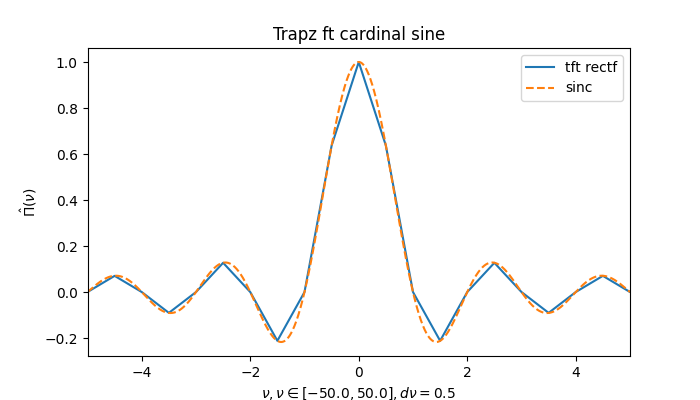
\includegraphics[width=\linewidth]{2_tftr.png}
            \caption{$\hat{\Pi}(t)$ восстановленной \texttt{trapz} $\Pi(t)$}
            \label{fig:tsinc2}
        \end{subfigure}
        \caption{Интеграл на уменьшенном промежутке от $-1$ до $1$}
        \label{fig:trapzs2}
    \end{figure}
    \vspace{-5mm}
    \begin{figure}[H]
        \centering
        \begin{subfigure}{0.45\textwidth}
            \centering
            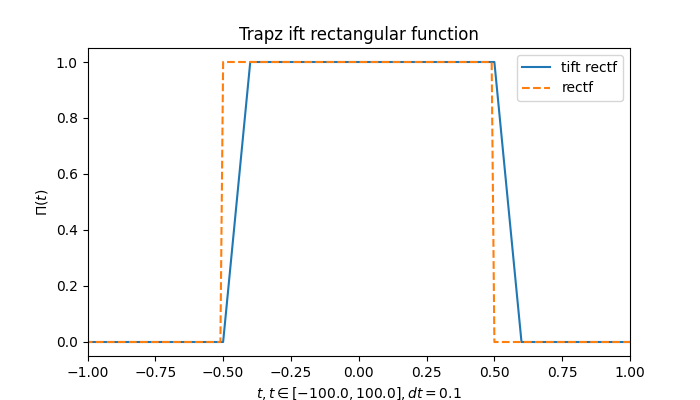
\includegraphics[width=\linewidth]{3_tiftr.png}
            \caption{$\Pi(t)$, восстановленная \texttt{trapz}}
            \label{fig:trectf3}
        \end{subfigure}
        \hspace{5mm}
        \begin{subfigure}{0.45\textwidth}
            \centering
            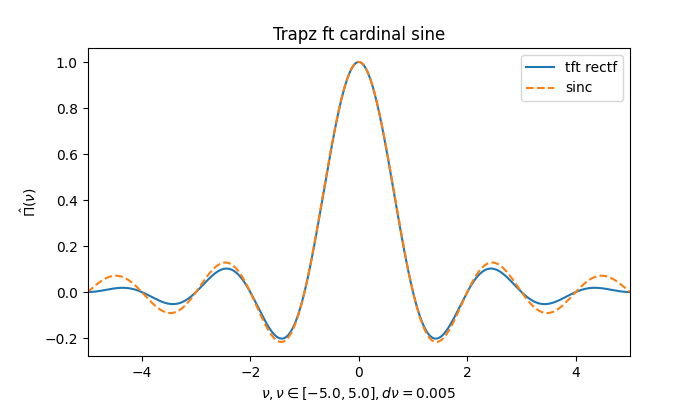
\includegraphics[width=\linewidth]{3_tftr.png}
            \caption{$\hat{\Pi}(t)$ восстановленной \texttt{trapz} $\Pi(t)$}
            \label{fig:tsinc3}
        \end{subfigure}
        \caption{Увеличение шага интегрирования $dt=0.1$, интеграл аналогично рис. \ref{fig:trapzs1}}
        \label{fig:trapzs3}
    \end{figure}
    \begin{figure}[H]
        \centering
        \begin{subfigure}{0.45\textwidth}
            \centering
            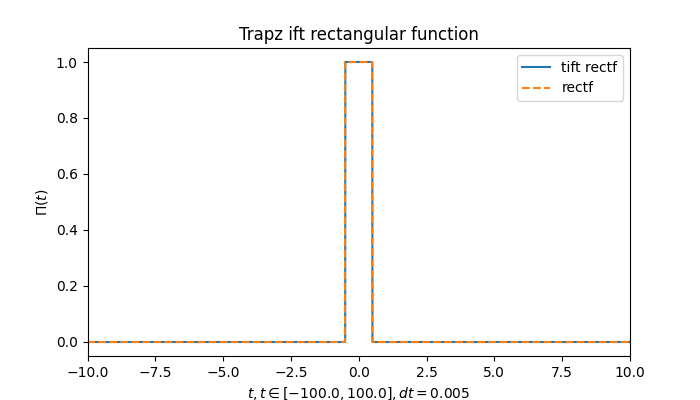
\includegraphics[width=\linewidth]{5_tiftr.png}
            \caption{$\Pi(t)$, восстановленная \texttt{trapz}}
            \label{fig:trectf5}
        \end{subfigure}
        \hspace{5mm}
        \begin{subfigure}{0.45\textwidth}
            \centering
            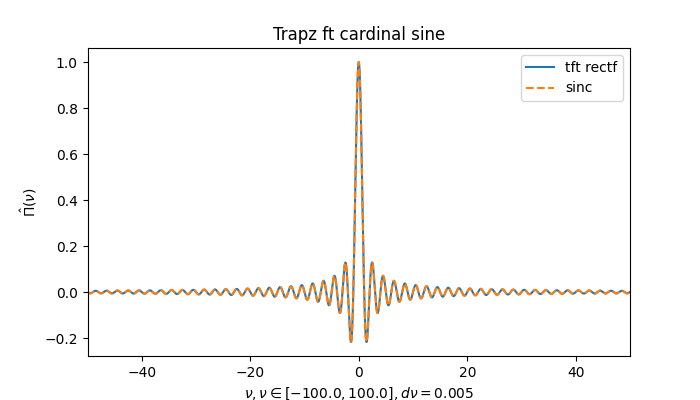
\includegraphics[width=\linewidth]{5_tftr.png}
            \caption{$\hat{\Pi}(t)$ восстановленной \texttt{trapz} $\Pi(t)$}
            \label{fig:tsinc5}
        \end{subfigure}
        \caption{Уменьшение шага интегрирования $dt=0.005$, интеграл аналогично рис. \ref{fig:trapzs1}}
        \label{fig:trapzs5}
    \end{figure}


    \subsection{Использование DFT}
    Найдем Фурье-образ функции $\Pi(t)$ с помощью дискретного преобразования Фурье (конструкция \texttt{fftshift(fft())}), используя его так,
    чтобы преобразование было унитарным. Выполним обратное преобразование от
    найденного Фурье-образа с помощью обратного дискретного преобразования (конструкция \texttt{ifft(ifftshift())}). Схематично наши действия можно представить так:
    \begin{center}
        $\Pi(t)$
        \begin{tikzpicture}
            \draw[->] (0,0) -- (2,0) node[midway, above] {\tiny{\texttt{fftshift(fft())}}};
        \end{tikzpicture}
        $\hat{\Pi}(\nu)$
        \begin{tikzpicture}
            \draw[->] (0,0) -- (2,0) node[midway, above] {\tiny{\texttt{ifft(ifftshift())}}};
        \end{tikzpicture}
        $\Pi(t)$
    \end{center}


    Для того, чтобы преобразование было унитарным, необходимо домножить ряд дискретного преобразования Фурье
    на коэффициент $1\div\sqrt{N}$. Аналогично для обратного преобразования Фурье. Таким образом, формулы DFT и IDFT будут
    иметь вид:
    $$
    \mathcal{F}_m = \dfrac{1}{\sqrt{N}}\sum\limits_{n=0}^{N-1}f_ne^{-2\pi i \frac{mn}{N}},\ \ f_n=\dfrac{1}{\sqrt{N}}\sum\limits_{m=0}^{N-1}\mathcal{F}_me^{2\pi i\frac{mn}{N}}
    $$
    Далее приведены сравнительные графики найденной $\hat{\Pi}(\nu)$ и восстановленной $\Pi(t)$ функций с исходными. Цвета и обозначения аналогичны предыдущему пункту.
    \begin{figure}[H]
        \centering
        \begin{subfigure}{0.45\textwidth}
            \centering
            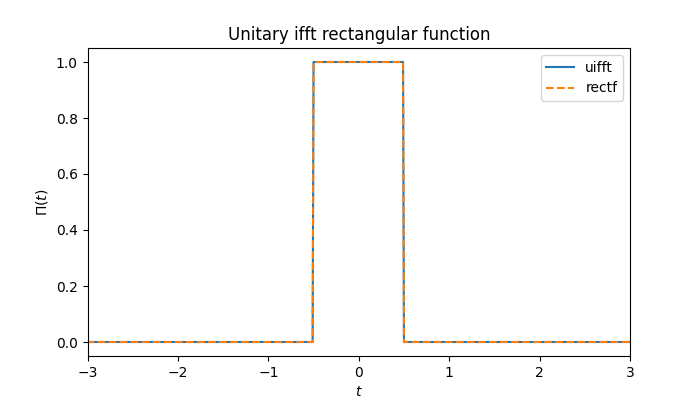
\includegraphics[width=\linewidth]{uifft.png}
            \caption{$\Pi(t)$, восстановленная \texttt{ufft}}
            \label{fig:uifft}
        \end{subfigure}
        \hspace{5mm}
        \begin{subfigure}{0.45\textwidth}
            \centering
            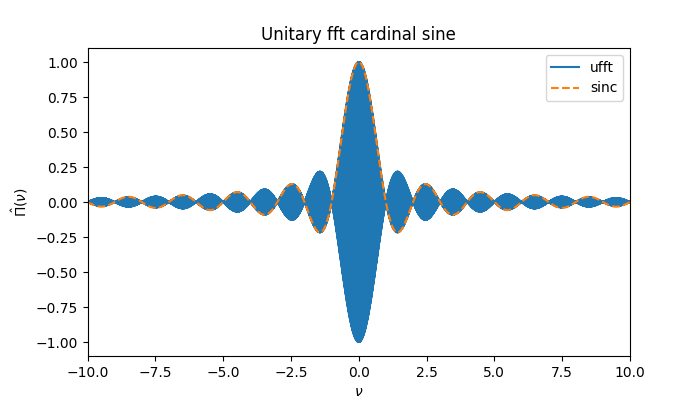
\includegraphics[width=\linewidth]{ufft.png}
            \caption{$\hat{\Pi}(t)$ восстановленной \texttt{ufft} $\Pi(t)$}
            \label{fig:ufft}
        \end{subfigure}
        \caption{Унитарное быстрое преобразование Фурье \texttt{ufft}}
        \label{fig:uffts}
    \end{figure}


    \subsection{Выводы о trapz и fft}
    объяснить


    \subsection{Приближение непрерывного с помощью DFT}
\end{document}